\documentclass{report}

\usepackage[utf8]{inputenc}  
\usepackage[T1]{fontenc}    
\usepackage{graphicx}
\usepackage{listings}

\makeatletter
\DeclareRobustCommand*\textsubscript[1]{%
  \@textsubscript{\selectfont#1}}
\def\@textsubscript#1{%
  {\m@th\ensuremath{_{\mbox{\fontsize\sf@size\z@#1}}}}}
\makeatother


\lstset{
  language=Caml
}

\title{TER - Rendu 1}
\author{Valentin Bouziat, Emile Cadorel, Jimmy Furet, Guillaume Gas}
\date{20 mai 2016}

\begin{document}
\maketitle

\chapter{Introduction}
Dans le cadre de notre projet de TER à l’Université d’Orléans, nous avons eu pour objectif de réaliser un module, pour la bibliothèque SPOC, de squelettes pour la programmation GPGPU à l’aide du langage OCaml.

\section{La Programmation GPGPU}
La programmation GPGPU\cite{refProgGPGPU} (General Purpose on Graphic Processing Units), est un principe informatique visant à utiliser le processeur graphique comme processeur de calcul générique. L’objectif étant de bénéficier de l’architecture massivement parallèle d’un processeur graphique et ainsi résoudre des problèmes pour lesquels nous avons des algorithmes parallèles efficaces.\newline \newline

\begin{figure}[!h]
\begin{center}
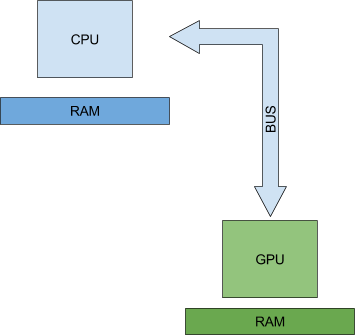
\includegraphics[height=150pt]{images_finales/image1.png}
\end{center}
\caption{Figure 1. Représentation simplifiée d'un ordinateur classique}
\label{test1}
\end{figure}

En effet le processeur graphique possède une capacité de calcul beaucoup plus grande que celle d’un processeur classique. Pour peu qu’il existe un algorithme parallèle pour un problème donné. La programmation GPGPU n’est applicable qu’avec utilisation des pilotes et des bibliothèques associées. Ces pilotes et bibliothèques généralement proposés par les constructeurs de processeur (ex: Intel, Nvidia, …) permettent la programmation sur la carte graphique pour des informaticiens chevronnés.\newline 

La programmation GPGPU optimise donc la puissance de calcul grâce à la parallélisation. Généralement, un algorithme exécuté en parallèle (en utilisant le processeur graphique ou plusieurs coeurs d'un processeur) terminera plus rapidement qu'un algorithme executé de manière séquentielle (sans se soucier de la parallélisation).  \newline

Le GPU possède une architecture SIMD (Single Instruction Multiple Data), proposant de nombreuses unités de calcul. \newline

Le GPU est découpé en plusieurs TCP (Texture Processing Cluster), eux-même découpés en plusieurs SM. Les SM (Streaming Multi-processor) possèdent une mémoire locale, ils possèdent plusieurs SP (Streaming Processor) permettant des calculs sur nombres flottants, ainsi que des unités SFU (Special Function) permettant le calcul de fonctions spécifiques (cos, sin...). Une mémoire globale est à la disposition de chacun des clusters mais et beaucoup plus lente que leur mémoire locale. \newline

\begin{figure}[!h]
\begin{center}
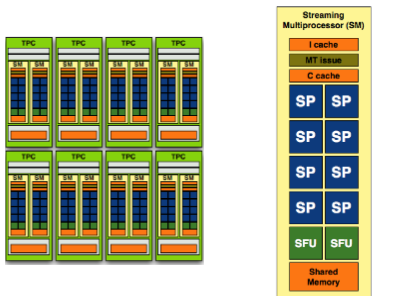
\includegraphics[height=150pt]{images_finales/image2.png}
\end{center}
\caption{Figure 2. Représentation d'une architecture GPU - ref : Introduction à la programmation GPGPU avec Cuda, Mathias Bourgoin, Sylvain Jubertie}
\label{test2}
\end{figure}

L'architecture d'un GPU étant SIMD, il n'est pas conseillé de créer des programmes complexes proposant beaucoup de conditions, ce qui ferait perdre l'intérêt parallèle de la carte, en effet, certains coeurs serait en attente la plupart du temps.

\section{Le langage OCaml}
Langage développé par l'INRIA (Institut National de Recherche Informatique et Automatique) anciennement connu sous le nom d'Objective Caml.\newline

OCaml est un langage multi-paradigme, c'est à dire qu'il permet l'utilisation de plusieurs paradigme de programmation tels que la programmation orientée objet ou encore la programmation statique. 

OCaml est un langage sûr, notamment grâce au typage fort et à sa gestion automatique de la mémoire. 

De plus, OCaml se distingue de la plupart des autres langages de programmation dans les milieux académiques pour ses excelentes performances. 

\section{SPOC}
SPOC\cite{refSpoc}, Stream Processing with OCaml est une bibliothèque qui propose une abstraction pour la programmation GPGPU. Son principal but est de fournir une solution portable, multi-GPGPU, et hétérogène tout en gardant de hautes performances.\newline

Elle permet ainsi l’utilisation des systèmes Cuda/OpenCL avec OCaml, l’unification de ces deux API se faisant via une liaison dynamique, ainsi que d’abstraire également les transferts de données entre le CPU et la carte graphique.\newline

Enfin, elle permet aussi d’utiliser le typage statique afin de vérifier les noyaux de calcul, écrits en Sarek.\newline

Il existe deux solutions afin d’exprimer les noyaux :
\begin{itemize}
  
\item Sarek : un langage proche de OCaml. Sarek est compatible avec les bibliothèques existantes, ses performances sont facilement prévisibles et optimisables.
  
\item L’interopérabilité avec les noyaux Cuda/OpenCL : permet de réaliser des optimisations supplémentaires, compatible avec les bibliothèques actuelles, mais moins robuste que Sarek.

\end{itemize}
  
\section{Les Squelettes de programmation}

Les squelettes de programmation\cite{refSkeleton} sont une forme de programmation, ou il existe des éléments générique pré-définis - tel que map, reduce, farm, pipe etc... Ces squelettes peuvent être personnalisés grâce à du code utilisateur.\newline

Les squelettes permettent une abstraction de haut niveau et aident les utilisateurs à implémenter des algorithmes complexe comme les algorithmes parallèles. Les algorithmes suivant sont généralement implémenté en tant que squelette dans les bibliothèque de programmation GPGPU.\newline

Afin de mieux comprendre le but de notre travail, nous avons fait des recherches sur la programmation de tels squelettes sur internet. Nous avons ainsi pris exemple sur deux bibliothèques qui semblent reprendre les concepts nous intéressent : Thrust, développée par Nvidia, et SkePU.\newline



\section{Objectifs et Organisation}
\subsection{Objectifs}
Les objectifs de ce projet peuvent se résumer en quatre principaux points :
\begin{itemize}
\item Comprendre et prendre en main la bibliothèque SPOC et Sarek.
\item Rechercher dans la littérature les types de squelettes intéressants à développer  pour des architectures hétérogènes.
\item Implémenter la bibliothèque de squelettes pour le langage OCaml avec SPOC.
\item Evaluer les performances obtenues sur des exemples en les comparant à une exécution séquentielle ainsi qu'à d'autres outils semblables issues de la littérature. 
\end{itemize}

\subsection{Organisation}

Nous avons tout d'abord fait des recherches sur les squelettes existant et réfléchit à la manière d'en intégrer à SPOC.\newline
Nous nous sommes alors partagé les tâches, certains travaillant sur la création de fonctions nécessaires à la création de squalettes, d'autres réalisant les squelettes.\newline

Afin de discuter de l'avancement du projet, nous avons régulièrement organisé des réunions, en personne ou par visio-conférences) avec notre tuteur et avons également dialogué par mail.\newline

Cela nous a permis de tenir notre tuteur au courant de notre avancement et de poser régulièrement des questions sur le fonctionnement de SPOC ou encore sur le langage OCaml en lui même.\newline

Nous avons également utilisé un dépôt pour y ajouter régulièrement notre code et afin de profiter de la force du logiciel de versionnage git.\newline
Lien du dépôt : https://github.com/USSEnterpriseTeam/USS

\chapter{Travaux effectués}
\section{Analyse de l'existant}
\subsection{Bibliothèques de programmation GPGPU existantes}

En matière de programmation GPGPU, les deux API les plus complètes sont Cuda et OpenCL.
\subsubsection{Cuda}

Cuda (Compute Unified Device Architecture) est une API de haut niveau proposant une architecture de traitement parallèle.\newline

L'API Cuda est développée par Nvidia (un des meilleurs fournisseurs de composants graphiques) et est d'ailleurs incluse dans la plupart de leurs produits, notamment les GPU GeForce et Ion Quadro.\newline

Cuda inclut des extensions C, C++ et Fortran qui permettent l'expression de calculs de données importantes et/ou complexes.\newline
Ces trois langages peuvent êtres utilisés simultanément pour l'expression des fonctions et des kernels.\newline

Cuda propose donc un accès standardisé à la puissance de calcul et a été très bien accueillie par la communauté scientifique. De plus, on retrouve l'utilisation de cette API dans plusieurs domaines notamment la recherche pharmaceutique : Cuda est utilisé et accélère Amber, logiciel de simulation moléculaire utilisé par plus de 60 000 chercheurs.\newline

Cuda est également accessible au public depuis Windows 7, les GPU de Nvidia ne sont désormais plus seulement des processeurs graphiques mais peuvent désormais faire office de processeurs de calcul parallèle. \newline

\subsection{Fonctionnement de Cuda}

Le fonctionnement de l'API Cuda nous permet de mieux comprendre les principes de la programmation GPGPU. \newline

\begin{figure}[!h]
\begin{center}
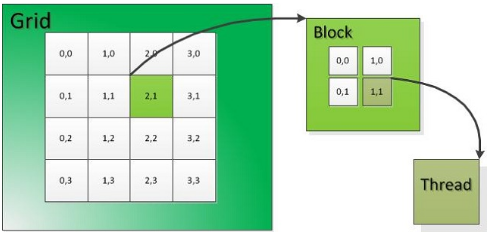
\includegraphics[height=150pt]{images_finales/image_cuda.png}
\end{center}
\caption{Organisation des threads sur une carte graphique Nvidia}
\label{test3}
\end{figure}

Une grille est constituée de blocs. Chaque bloc est constitué de threads. Les blocs sont des éléments des calculs dissociables les uns des autres. Ils peuvent être exécutés dans un ordre aléatoire, le plus parallèle possible à la décision du driver de la machine exécutrice. C'est pourquoi chaque thread ne peut communiquer qu'avec les threads d'un même bloc.\newline

Un warp est un ensemble de 32 threads, envoyés ensemble à l'exécution et executés simultanément. Un thread est exécuté par un processeur (un des coeurs de GPU), on peut donc établir une correspondance entre le thread et une unité de calcule séquentielle.\newline
Ainsi, le bloc est le multiprocesseur, tandis que la grille représente l'entièreté de la carte graphique. \newline

Il est possible à l'utilisateur de faire varier le nombre de blocs et de threads utilisés dans le calcul parallèle. Il est donc primordiale lors de la programmation d'un kernel de se soucier du nombre de blocs et de threads à utiliser en fonction de plusieurs paramètres (capacités de la carte graphique, bon compromis entre nombre de blocs et de threads). \newline

\subsubsection{OpenCL}

OpenCL (Open Computing Language) est la combinaison d'une API pour le calcul parallèle et d'un langage dérivé du C. Initiallement créé par Apple puis racheté par le groupe Khronos, ce langage est de plus bas niveau comparé à Cuda. \newline

OpenCL permet l'exécution de programmes parallèles sur plusieurs processeurs graphiques de constructeurs différents. \newline

Contrairement à Cuda, OpenCL a été conçu pour exécuter des calculs parallèles pas seulement sur des processeurs graphiques, mais aussi sur des CPU multi-coeurs. \newline

\subsection{Analyse de SPOC}

Pour mener à bien notre travail, nous avons dû étudier minutieusement SPOC et ses composants afin de comprendre comment cette bibliothèque fonctionne. Il faut savoir que la bibliothèque SPOC est très peu documentée et que nous n'avions pas de connaissances en OCaml.\newline
Malgré tout, nous nous sommes vite familiarisé avec le compilateur Sarek, composant de SPOC, afin d'implémenter correctement nos squelettes. \newline

\subsubsection{Fonctionnement général de SPOC}

SPOC permet principalement l'intéropérabilité Cuda/OpenCL :\newline

SPOC détecte, dans un premier temps, les différents processeurs de calcul parallèle accessibles depuis l'hôte.\newline
Ensuite, les calculs à exécuter en parallèle sont réparties sur les différents processeurs de calcul (en utilisant Cuda pour les GPU Nvidia ou OpenCL pour les autres GPU ou les CPU multi-coeurs). \newline

Pour ce faire, SPOC propose un langage de programmation appelé Sarek. Ce langage permet à un utilisateur ne connaissant ni Cuda, ni OpenCL, de créer ses propres kernels dans un langage proche de OCaml. Ces morceaux de programme sont ensuite analysés à la compilation afin de générer un arbre de syntaxe, et d'effectuer une vérification des types.\newline

Ces arbres de syntaxe sont ensuite récupérés à l'exécution du programme et compilés dans le langage cible (le C), pour Cuda ou OpenCL, suivant l'architecture de la machine exécutrice. \newline

\subsection{Squelettes de programmation existants}

Nous avons ainsi pris exemple sur deux bibliothèques qui semblent reprendre les concepts nous intéressant : Thrust, développée par Nvidia, et SkePU.

\subsubsection{Thrust}

Cette bibliothèque de templates C++ pour Cuda est basée sur la STL (Standard Template Library). Elle permet l’utilisation d’algorithmes parallèles avec un minimum de code. Ainsi, on retrouve les algorithmes suivant :

\begin{itemize}
\item Transformations : applique une opération d’un “set” de données et met le résultat dans un “set” de destination. 
\item Réductions : utilise une opération binaire pour réduire une entrée en une unique valeur. 
\item Prefix-Sums : ou opération “scan” permet par exemple, sur un tableau en entrée, d’obtenir en sortie un tableau avec les sommes cumulées.
\item Reordering : permet d’arranger ou partitionner des données selon des prédicats de test.
\item Sort : tri un ensemble d’élément à l’aide d’une relation d’ordre donné.
\end{itemize}

\subsubsection{SkePU}

Librairie de templates C++ mettant à disposition un ensemble de squelettes génériques.

\begin{itemize}
\item Map\cite{refMap} - applique une fonction donnée à toutes les entrées d’un tableau.
\item MapReduce - réduction d’un tableau dans une variable, en fonction d’un operateur donné.
\item MapOverlap (ou Stencil)
\item MapArray
\item Generate
\item Scan
\end{itemize}

Nous nous sommes inspirés à de nombreuses reprises des squelettes présents dans ces deux bibliothèques pour implémenter nos propres squelettes en OCaml et les inclures à SPOC.

\newpage
\section{Implémentation des squelettes}

Afin d'implémenter nos différents squelettes, nous avons créé un module OCaml Skeleton regroupant les différentes fonctions nécessaires à la création d'un kernel à partir d'un squelette, ainsi que les différents squelettes implémentés. 

\subsection{Génération des kernels}

Comme nous l'avons vu précédemment, SPOC permet de créer des kernels, Cuda ou OpenCL, à partir d'un arbre de syntaxe (AST) à partir du moment où celui-ci est correctement typé. En temps normal, cet AST est le résultat de la compilation de Sarek, dans notre cas la situation était un peu différente. Notre objectif a été de récupérer un arbre de syntaxe généré par l'utilisateur afin de l'implanter dans un kernel et de compiler l'arbre obtenu, pour ce faire il a fallu rajouter des éléments dans l'arbre de syntaxe de Sarek.\newline

Le premier élément que nous avons ajouté est le noeud \textit{Skel}, ce noeud est une balise qui est ensuite interprétée comme un appel de fonction \textit{inline}. Il contient une liste de paramètres et un paramètre de retour. \newline

\begin{lstlisting}
Skel (a, b, c) -> d
\end{lstlisting}

C'est grâce à ce noeud que nos squelettes peuvent être modulaires et permettent à l'utilisateur d'établir des critères sur le fonctionnement de l'algorithme. Par exemple, pour un tri, l'utilisateur peut vouloir trier son tableau de manière décroissante, il va donc passer une fonction de test à l'algorithme. Celle-ci prend deux paramètres et renvoie vrai si le premier est plus grand que le deuxième. Ainsi, le noeud Skel est remplacé par la fonction de l'utilisateur et le test est correctement effectué. 

\begin{figure}[!h]
\begin{center}
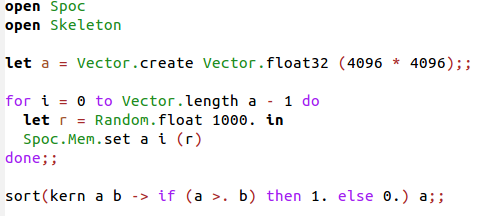
\includegraphics[height=150pt]{images_finales/sort.png}
\end{center}
\caption{Figure 5. Appel du squelette de tri pour l'utilisateur}
\label{test5}
\end{figure}

Pour permettre d'exécuter des algorithmes, comme le tri, il a fallu générer des arbres de syntaxe qui contiennent le code voulu avec les noeuds \textit{Skel}. Ces noeuds ne faisant pas partie directement de la grammaire de Sarek, ils ne peuvent pas être analysés par son analyseur syntaxique, il a donc fallu les écrire à la main. \newline

Une fois nos AST de squelettes créés, ils sont envoyés dans une routine qui va les transformer en arbre de syntaxe correctement typé et ne contenant que des noeuds transformables par le générateur de code de Sarek.\newline

\begin{figure}[!h]
\begin{center}
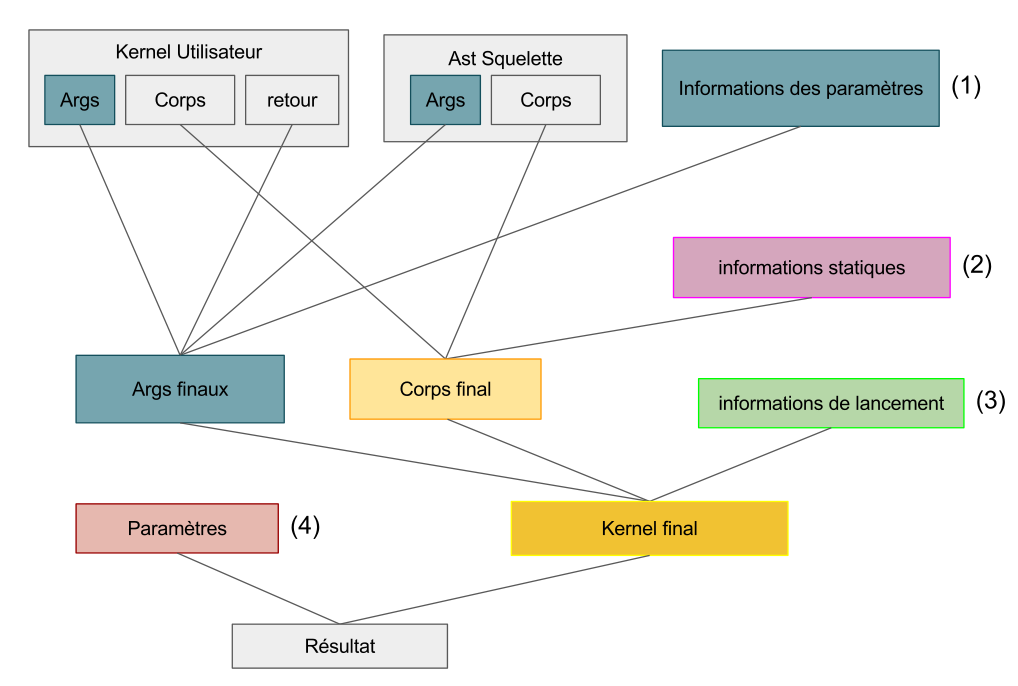
\includegraphics[height=150pt]{images_finales/fonctionnement_skel.png}
\end{center}
\caption{Figure 6. Représentation graphique de la transformation des squelettes en kernels exécutables}
\label{test6}
\end{figure}

Nous voyons donc dans ce schéma le kernel de l'utilisateur, qui peut être par exemple la fonction de test pour un tri, l'AST du squelette et quelques autres informations. \newline

\begin{enumerate}
\item Les informations sur les paramètres : 
La première information va concerner le type des paramètres du kernel final. Il est structuré sous la forme d'une liste qui fait la taille des paramètres du squelette et spécifie à chacun d'eux le type qu'ils doivent avoir. Cette liste est générée en fonction des types des paramètres du kernel de l'utilisateur, du type de retour de ce kernel, ainsi que de certaines contraintes imposées par l'algorithme (exemple: le tri prend en entrée un tableau, mais l'utilisateur va prendre uniquement deux flotants). \newline

\item Les informations statiques : 
Les informations statiques peuvent être vues comme des macros, elles vont permettre de modifier quelques éléments de l'AST qui vont permettre à l'algorithme de s'exécuter correctement. Elles sont enregistrées sous la forme d'une liste qui peut contenir tout type d'informations. Comme le remplacement d'une variable par une constante, la modification du type d'une variable... \newline

\item Les informations de lancement : 
Ces informations n'interviennent pas au moment de la génération du kernel, mais au moment de l'exécution. Elles permettent de connaître les paramètres qui sont donnés par l'utilisateur et de générer ceux qui ne le sont pas. Par exemple, l'information de sortie est renvoyée par le kernel Cuda ou OpenCL par effet de bord, il faut donc créer un paramètre qui va être en fait la sortie de ce kernel. \newline

\item Les paramètres : 
Les paramètres contenus dans ces informations sont uniquement ceux passés par l'utilisateur, les autres vont être générés par la routine de lancement grâce aux informations de lancement vues au paragraphe précédent. \newline
\end{enumerate}

Nous venons de voir comment l'utilisateur peut appeler un squelette. Le squelette en question est le suivant : \newline

\begin{figure}[!h]
\begin{center}
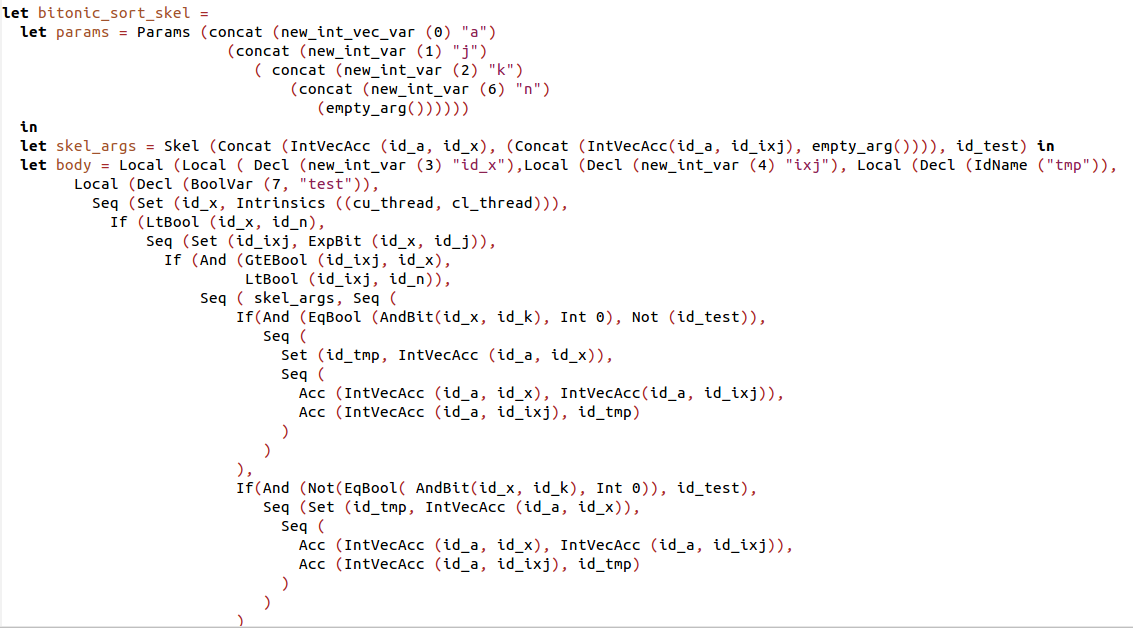
\includegraphics[height=150pt]{images_finales/skel_sort.png}
\end{center}
\caption{Figure 7. Code du squelette du bitonic sort}
\label{test7}
\end{figure}

\newpage
Le squelette de l'AST de l'utilisateur est ensuite envoyé dans la routine de transformation pour générer le code suivant (ici en OpenCL) : \newline

\begin{figure}[!h]
\begin{center}
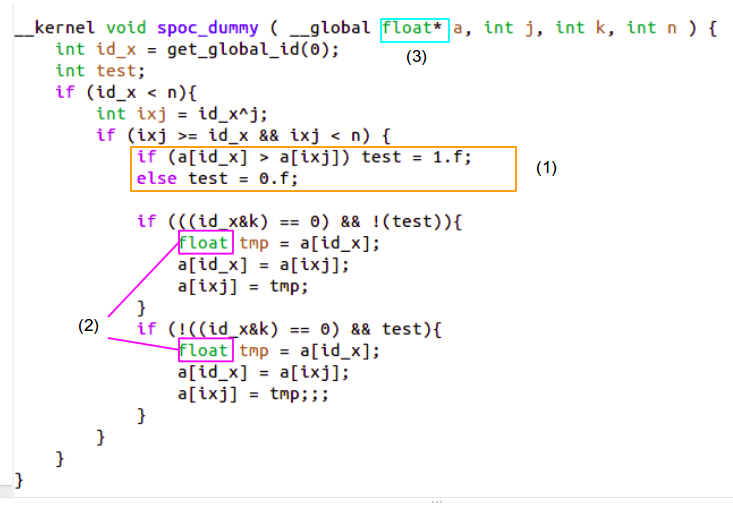
\includegraphics[height=150pt]{images_finales/kernel_sort.png}
\end{center}
\caption{Figure 8. Kernel généré à partir du squelette du bitonic sort}
\label{test8}
\end{figure}


\begin{enumerate}
\item Remplacement du noeud Skel
\item Remplacement statique en fonction du type de l'utilisateur
\item Type de l'utilisateur
\end{enumerate}
\newpage
\subsection{Squelettes implémentés}
\subsubsection{Map}

Le \textit{Map} est un algorithme classique dans la programmation GPGPU. Il est facilement parallélisable étant donné que son objectif est d'appliquer une opération à chacune des cases d'un tableau.\newline

\begin{lstlisting} 
Entree : un tableau T
Sortie : un tableau S
Pour Tout i dans T
    S[i] = f(T[i])
\end{lstlisting}

\subsubsection{Reduce}

L'objectif d'un \textit{Reduce} est de réduire un tableau dans une seule variables afin d'en avoir la somme, le produit...\newline

L'algorithme du \textit{Reduce} utilise la mémoire partagée afin de permettre une optimisation des accès mémoire ainsi qu'une communication entre les threads d'un même bloc.\newline

L'algorithme du \textit{Reduce} fonctionne de la manière suivante : les données sont tout d'abord placées en mémoire partagée. Chaque bloc effectue alors l'opération du \textit{Reduce} sur sa mémoire partagée de la façon suivante (exemple avec une somme) : \newline
\begin{center}
\end{center}
\begin{figure}[!h]
\begin{center}
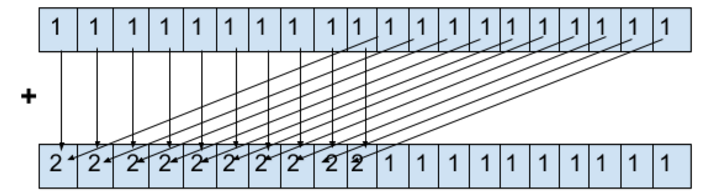
\includegraphics[width=250pt]{images_finales/schema_reduce.png}
\end{center}
\caption{Exemple d'une première étape de l'algorithme du reduce}
\label{test9}
\end{figure}

Cette opération est répétée jusqu'à avoir le résultat du \textit{reduce} local au bloc dans la première case de la mémoire partagée au bloc.\newline

L'algorithme est appelé deux fois, la première fois le tableau de résultats contient le résultat de chacun des N blocs et fais une taille de N. La deuxième fois, l'algorithme est appelé avec uniquement un seul bloc, de cette façon le résultat du \textit{Reduce} est dans la première case du tableau.\newline

Vous trouverez ici une version de l'algorithme écrit en C++ avec Cuda et effectuant une somme : \newline
 
\begin{figure}[!h]
\begin{center}
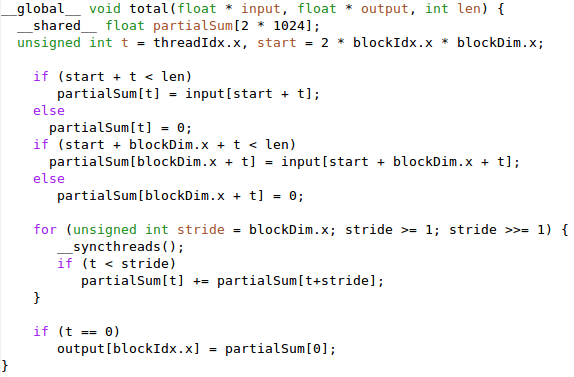
\includegraphics[height=130pt]{images_finales/reduce.png}
\end{center}
\caption{Figure 10. Kernel Cuda du Reduce}
\label{test10}
\end{figure}

\subsubsection{Stencil}
Les algorithmes \textit{Stencil} sont une catégorie d'algorithme parallèle qui mettent à jour un tableau d'éléments en fonction d'un pattern. Dans notre cas, le \textit{Stencil} est appliqué à un tableau une dimension, et l'utilisateur peut spécifier l'opération à appliquer ainsi que la taille du pattern. Le code en OpenCL est le suivant :\newline

\begin{figure}[!h]
\begin{center}
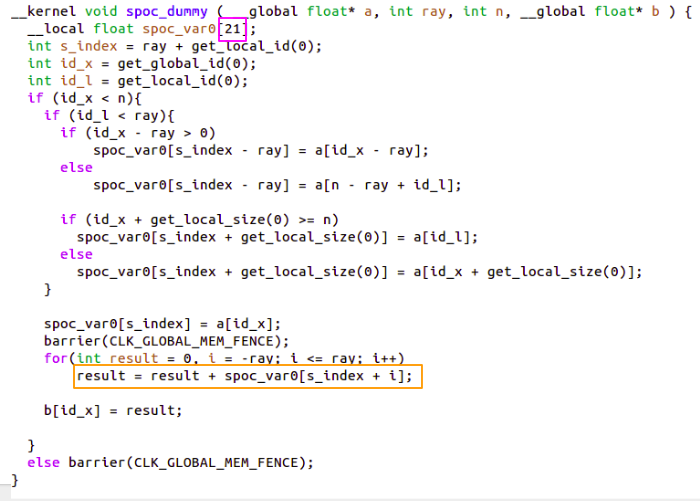
\includegraphics[height=130pt]{images_finales/Stencil_kernel.png}
\end{center}
\caption{Figure 11. Code OpenCL d'un kernel de Stencil. \textit{En violet, nombre de thread+rayon*2 (emplacement statique à la génération), en jaune, la fonction utilisateur}}
\label{test11}
\end{figure}
\newpage

Le kernel de la figure 10 a été générée par un squelette de \textit{Stencil} auquel on a appliqué une règle d'addition et un rayon de 2. Pour chaque case \textit{i} de ce tableau, le kernel généré additionne les 2 cases qui précédent \textit{i}, et les 2 cases qui suivent \textit{i} (car le rayon est égale à 2), ainsi que la valeur initiale de la case : \newline

\begin{figure}[!h]
\begin{center}
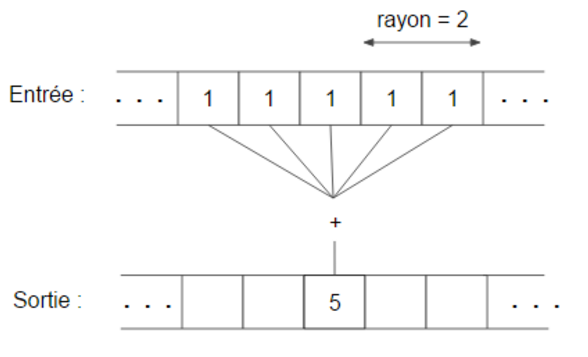
\includegraphics[height=150pt]{images_finales/schema_stencil.png}
\end{center}
\caption{Figure 12. Schéma d'une étape de l'application de l'algorithme du Stencil}
\label{test12}
\end{figure}

\subsubsection{Generate}

L'algorithme de \textit{Generate} est un algorithme très simple qui remplis un tableau à partir d'un pattern. \newline

\begin{lstlisting} 
Entree : une taille N
Sortie : un tableau S
Pour i Allant de 0 a N
    S[i] = f(i)
\end{lstlisting}

\subsubsection{Bitonic Sort}

Le tri bitonique est un tri qui est bien applicable à la parallélisation. Cet algorithme est basé sur une fonction appelé fusionneur. Un fusionneur à N entrées a pour propriété que si les entrées (a\textsubscript{0}, ..., a\textsubscript{N/2}) et (a\textsubscript{N/2+1}, ..., a\textsubscript{N}) sont triées alors la sortie (b\textsubscript{0}, ..., b\textsubscript{N}) est trié.\newline

Le fusionneur est la partie de l'algorithme qui peut être parallélisée et est donc exécuté par une kernel.\newline

Ce kernel est appelé log\textsubscript{2}(N) fois par le CPU, avec N la taille du tableau d'entrée, afin que tout le tableau soit trié. Un inconvénient de cet algorithme est qu'il est obligatoire que l'entrée soit d'une taille en puissance de 2. \newline

\begin{figure}[!h]
\begin{center}
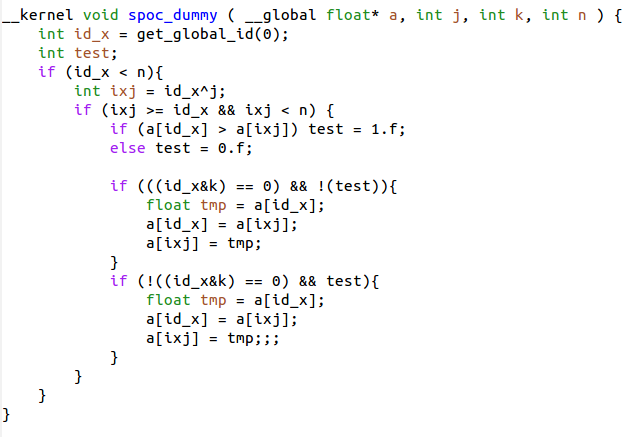
\includegraphics[height=150pt]{images_finales/kernel_sort_clean.png}
\end{center}
\caption{Figure 13. Fusionneur utilisé comme kernel}
\label{test13}
\end{figure}


\subsection{Rapports de performance}
Nous avons réalisé des rapports de performances pour justifier l'efficacité de nos algorithmes parallèles.\newline

Exécution sur : \newline
\begin{itemize}
\item Mémoire vive 1.9 Go
\item Intel Celeron CPU N3050 1.6Ghz * 2
\item Intel HD Graphics (CherryView)
\end{itemize}

Voici un premier benchmark de notre tri-bitonique en OpenCL sur un processeur graphique intégré : \newline
\begin{center}
  \begin{tabular}{|*{3}{c|}}
    \hline
    Taille du tableau d'entrée &  Exécution séquentielle (s) & Excécution parallèle (s) \\
    \hline
    4096 &  0.00872 & 0.007129 \\
    \hline
    8192 & 0.0176 & 0.0145 \\
    \hline
    262144 & 0.433 & 0.199 \\
    \hline
    8288608 & 15.052 & 9.888 \\
    \hline
    16777216 & 29.872 & 19.299 \\
    \hline
  \end{tabular}
\end{center}

Sur carte graphique Nvidia (GT 720) et processeur i5 (4*1.6 Ghz), on arrive à un gain supérieur sur un tableau à 16777216 entrées de 2 secondes en parallèle contre 9 secondes en séquentiel.\newline

On constate qu'à mesure que la taille du tableau en entrée augmente, l'utilisation de nos algorithmes se distingue d'une utilisation séquentielle.\newline

Cependant, pour des valeurs plus petites (4096 et 8192), la parallélisation est plus lente puisqu'il faut rajouter une temps constant de 0.2 secondes pour la génération du kernel. Mais, à mesure que la taille du tableau augmente, nous pouvons considérer que le temps de génération du kernel est négligeable.\newline

Nous avons ensuite effectué un benchmark d'un generate suivie d'un map.\newline
\begin{figure}[!h]
\begin{center}
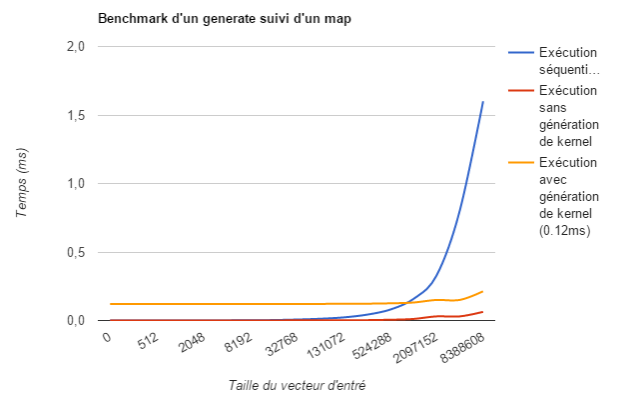
\includegraphics[height=100pt]{images_finales/benchmark.png}
\end{center}
\caption{Figure 14.}
\label{test14}
\end{figure}


On constate encore une fois que pour des tableaux de petite taille, une exécution parallèle est plus lente, du fait que la génération du kernel prend un temps constant et est donc handicapant pour ces cas.\newline

Cependant, l'exécution de ce kernel en parallèle devient beaucoup plus efficace qu'une exécution séquentielle au fur et à mesure qu'on augmente la taille du tableau en entrée. Ce qui permet d'être beaucoup plus performant sur des tableaux de grande taille.\newline

On peut aussi noter que si le kernel généré pouvait être sauvegardé plutôt que d'être généré à chaque exécution, on pourrait même rivaliser avec une exécution séquentielle sur des tableaux de petite taille.\newline

\chapter{Conclusion}
\section{Rappel du travail demandé}

Le projet a donc consisté à : \newline
\begin{itemize}
\item Comprendre et prendre en main la bibliothèque SPOC et Sarek.
\item Rechercher dans la littérature les types de squelettes intéressants à développer  pour des architectures hétérogènes.
\item Implémenter la bibliothèque de squelettes pour le langage OCaml avec SPOC.
\item Evaluer les performances obtenues sur des exemples en les comparant à une exécution séquentielle ainsi qu'à d'autres outils semblables issues de la littérature. 
\end{itemize}

\section{Travaux effectués}
Dans un premier temps, nous avons effectué des recherches sur les bibliothèques de squelettes existantes, les principes de la programmation GPGPU et les différentes bibliothèques permettant cette dernière.\newline

Ensuite, nous avons effectué des modifications au sein de SPOC pour permettre la création de nouveaux squelettes.\newline

Pour créer des squelettes pour SPOC, nous avons ajouté un module à SPOC, contenant les fonctions permettant l'appel à nos squelettes. Pour cela, nous avons ajouté différents éléments à l'arbre de syntaxe de Sarek, éléments qui sont ensuite remplacés par les fonctions créées par les utilisateurs de SPOC.\newline

Nos squelettes exécutent du code utilisateur de manière parallèle en générant des kernels compatibles avec SPOC.\newline

Nous avons effectué des tests de performance sur des calculs parallélisés en les comparant à une exécution séquentielle.\newline

Une brève documentation utilisateur pour nos squelettes est en cours de rédaction et devrait être bientôt accessible sur le dépôt du projet.\newline

\section{Améliorations possibles}
Il reste possible d'apporter des améliorations sur le projet SPOC, notamment l'ajout de squelettes supplémentaires (Scan, Pipe, Farm...).\newline

Une autre amélioration intéressante serait d'implémenter une bibliothèque de génération de squelettes pour pouvoir en ajouter plus facilement. Cette fonctionnalité reste néanmoins dans le domaine du concept et doit être étudiée plus en profondeur pour en véifier la faisabilité.\newline

Enfin, nos squelettes génèrent des kernels qui sont exécutés en parallèle, mais ces derniers dispairaissent après leur exécution. On pourrait donc imaginer un système de cache qui sauvegarde temporairement les kernels générés afin d'éviter de devoir les regénérer à chaque appel de squalette.\newline

\section{Apports pédagogiques}
Nous nous sommes familiarisés avec le langage OCaml, un langage que nous n'avions pas étudié jusqu'ici.\newline

De plus, ce projet nous a permis d'approfondir nos connaissances dans le domaine de la programmation GPGPU, que nous avons étudié au cours de cette année. \newline

Nous avons aussi beaucoup appris sur le concept de squelette de programmation ainsi que les nombreuses bibliothèque de squelettes existantes. Ces connaissances nous apportent une plus grande vision de ce domaine, ainsi qu'un approche plus ``logicielle'' de la programmation GPU.\newline

Enfin, nous avons bien sûr découvert l'existence de la bibliothèque que nous avons étudiée en détails, la bibliothèque SPOC.

\bibliographystyle{unsrt}
\bibliography{biblio}

\end{document}
